% Created 2018-10-08 Mon 15:40
% Intended LaTeX compiler: pdflatex
\documentclass[presentation,12pt]{beamer}
\usepackage[utf8]{inputenc}
\usepackage[T1]{fontenc}
\usepackage{graphicx}
\usepackage{grffile}
\usepackage{longtable}
\usepackage{wrapfig}
\usepackage{rotating}
\usepackage[normalem]{ulem}
\usepackage{amsmath}
\usepackage{textcomp}
\usepackage{amssymb}
\usepackage{capt-of}
\usepackage{hyperref}
\usetheme{Hannover}
\author{Matheus Artur, Luís Alberto Cabús, Nicolas Leão, Fábio Vinícius}
\date{\url{https://github.com/projetosufal/data-structures-project}}
\title{Segment Tree}
\hypersetup{
 pdfauthor={Matheus Artur, Luís Alberto Cabús, Nicolas Leão, Fábio Vinícius},
 pdftitle={Segment Tree},
 pdfkeywords={},
 pdfsubject={},
 pdfcreator={Emacs 26.1 (Org mode 9.1.9)}, 
 pdflang={English}}
\begin{document}

\maketitle
\begin{frame}{Outline}
\tableofcontents
\end{frame}


\section{Intro}
\label{sec:org2504831}

\begin{frame}[label={sec:org40c6638}]{Stock Exchange}
\begin{columns}
\begin{column}{0.48\columnwidth}
\begin{block}{The problem}
\begin{itemize}
\item Data from thousands of companies worldwide, active for decades
\item Usage of multiple operations requiring a range/interval of data in any capacity
\item Recources are not inifinite, must be optimized as best as possible
\end{itemize}
\end{block}
\end{column}


\begin{column}{0.48\columnwidth}
\begin{block}{O(n) operations? No!}
\begin{center}
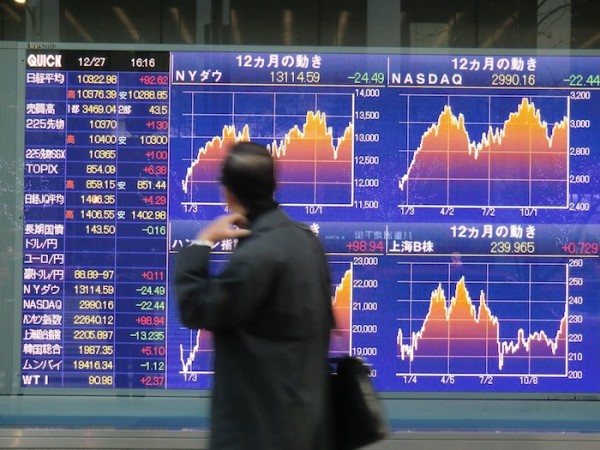
\includegraphics[width=.9\linewidth]{./img/serv.png}
\end{center}
\end{block}
\end{column}
\end{columns}
\end{frame}
\section{Segment tree}
\label{sec:orgf9892d7}
\begin{frame}[label={sec:org33dcb1a}]{Segment tree}
\begin{columns}
\begin{column}{0.48\columnwidth}
\begin{block}{How it is structured?}
\begin{itemize}
\item The Segtree is a binary tree that's represented from a array, where each node represents a unique interval or segment of the tree and stores a \alert{specific} value.
\item The value, is usually represented by \emph{maximum}, \emph{minimum} or \emph{sum} of the segment.
\end{itemize}
\end{block}
\end{column}
\begin{column}{0.48\columnwidth}
\begin{block}{Intervals of a A[6]}
\begin{center}
\begin{tabular}{lll}
\hline
tree[0] & = & A[0:5]\\
tree[1] & = & A[0:2]\\
tree[2] & = & A[3:5]\\
tree[3] & = & A[0:1]\\
tree[4] & = & A[2:2]\\
tree[5] & = & A[3:4]\\
tree[6] & = & A[5:5]\\
tree[7] & = & A[0:0]\\
tree[8] & = & A[1:1]\\
tree[9] & = & NULL\\
tree[10] & = & NULL\\
tree[11] & = & A[3:3]\\
tree[12] & = & A[4:4]\\
\hline
\end{tabular}
\end{center}
\end{block}
\end{column}
\end{columns}
\end{frame}
\begin{frame}[label={sec:org677df1e}]{As tree}
\begin{center}
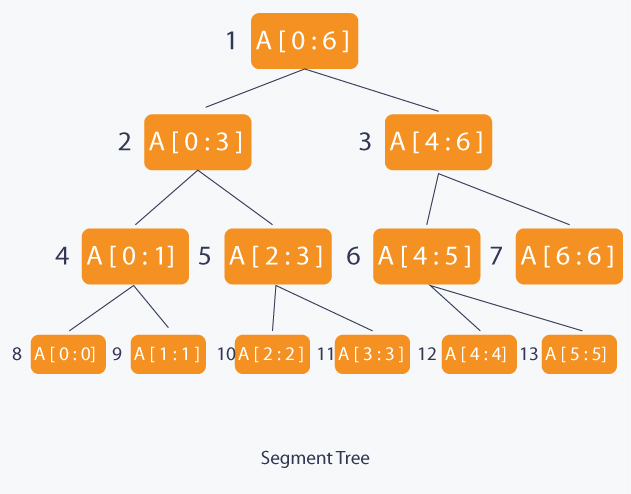
\includegraphics[width=.9\linewidth]{./img/segtree.jpg}
\end{center}
\end{frame}

\section{Operations}
\label{sec:org330fa8b}
\begin{frame}[label={sec:orgf316d2a}]{Operations}
\begin{block}{Building a tree}
\begin{itemize}
\item ( n log n) storage
\item but only (2*n - 1) actual nodes
\end{itemize}
\end{block}
\begin{block}{Query - range search}
\begin{itemize}
\item O(log n)
\end{itemize}
\end{block}
\begin{block}{Updating a tree}
\begin{itemize}
\item O(log n)
\item can modify any [l:r] section, than it will propagate updating dependencies
\end{itemize}
\end{block}
\end{frame}
\begin{frame}[label={sec:org9f2a104}]{Building a Segtree}
\begin{center}
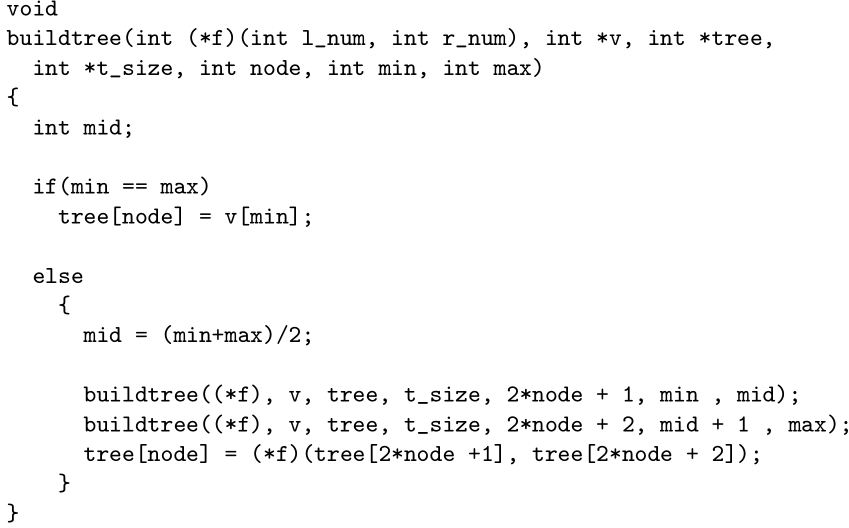
\includegraphics[width=.9\linewidth]{./img/build.png}
\end{center}
\end{frame}

\begin{frame}[label={sec:orgae0d997}]{Query}
\begin{center}
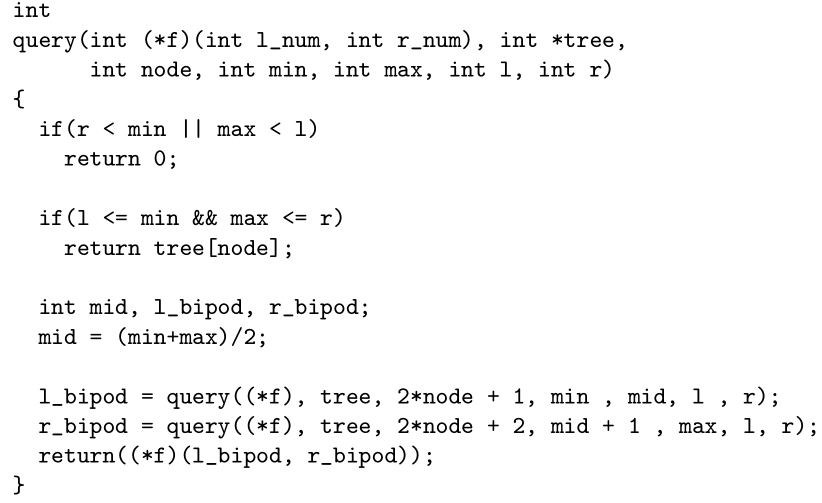
\includegraphics[width=.9\linewidth]{./img/query.png}
\end{center}
\end{frame}

\begin{frame}[label={sec:orgcf0faf5}]{Update}
\begin{center}
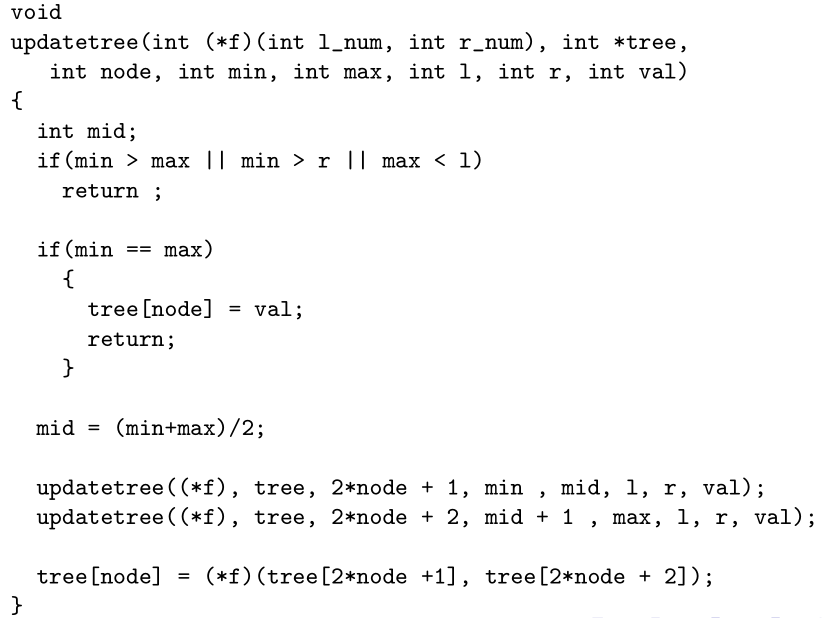
\includegraphics[width=.9\linewidth]{./img/update.png}
\end{center}
\end{frame}
\section{Peek: Segtree as a base for advanced algorithms}
\label{sec:orge61c458}
\begin{frame}[label={sec:org8b6ea4b}]{Segtree as a base for advanced algorithms}
As seen, segtree is a flexible algorithm, such power can be used as a base for even more advanced algorithms, such as Heavy Light Decomposition
\begin{itemize}
\item HLD takes segtree to another new level, transforming linear paths of the graph into multiple segtrees
\end{itemize}
\end{frame}
\begin{frame}[label={sec:org63cf378}]{Heavy Light Decomposition - a Segtree in graph}
\begin{center}
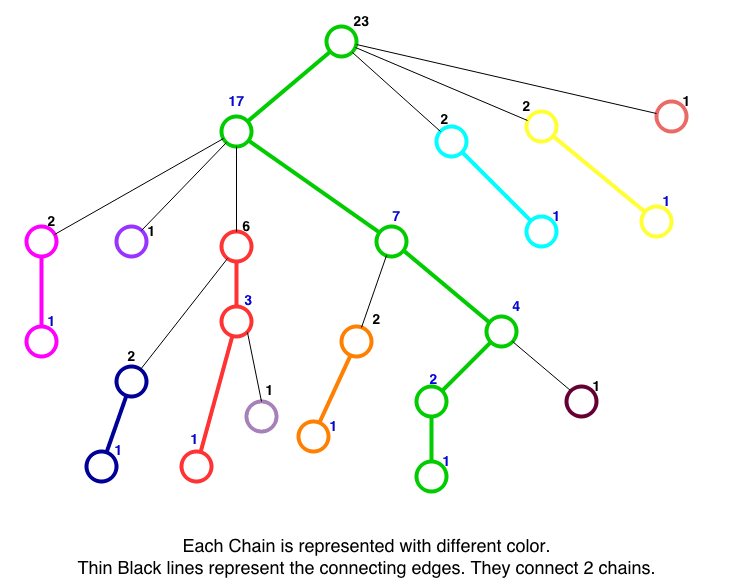
\includegraphics[width=.9\linewidth]{./img/hld.png}
\end{center}
\end{frame}
\section{Conclusion}
\label{sec:org2caf795}
\begin{frame}[label={sec:orgd18b086}]{Conclusion}
the algorithm is better suited to solve problems of:
\begin{itemize}
\item analysis of big chunks of data
\item reorganization and update of said data
\end{itemize}
And these properties are highly applicable in fields of stock market, weather analysis and competitive programming alike
\end{frame}
\end{document}
